\chapter{Control Software}

In order to control the whole automated assembly system a PC-based Qt~application was developed. All the necessary hardware is connected to the PC with USB interface.

\section{General structure of the application}

The control of the motion, vision and vacuum subsystems is integrated in a single software application henceforth referred to as PSAuto (from automated assembly of PS module). It is entirely written in C++ and utilises the Qt~framework version~4.8.7. A schematic illustrating the integration of the subsystems with PSAuto is shown in Figure \ref{fig:general_app_structure}.

\begin{figure}[ht]\centering
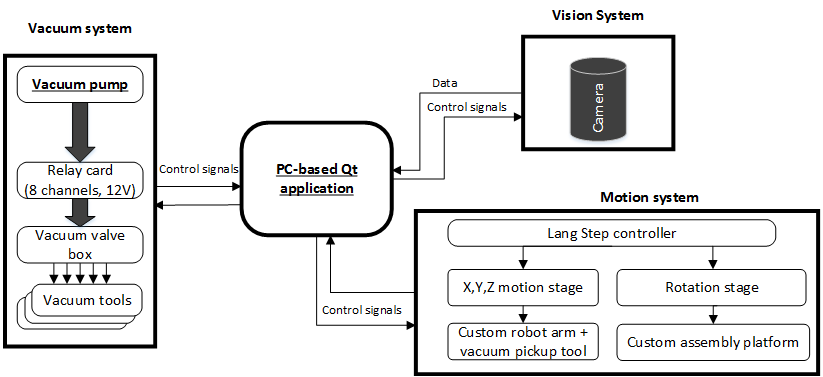
\includegraphics[width=1\linewidth]{Data/Control_Software/Whole_system_diagram_(English).png}
\caption{A schematic view of the integration of the motion, vision and vacuum subsytems via the Qt-application.}
\label{fig:general_app_structure}
\end{figure}



\subsection{Model View Controller architectural pattern}

The architecture of the application is based on Model-View-Controller (MVC) architectural pattern. It considers there to be three main types of objects: model objects, view objects and controller objects. When designing an application, a major step is choosing or creating custom classes for objects that fall into one of these three groups. Each of the three types of objects is separated from the others by abstract boundaries and communicates with objects of the other types across those boundaries. The pattern defines not only the roles objects play in the application, it also defines the way objects communicate with each other \cite{apple_MVC}. The key point of MVC is that View and Controller depend on Model, but Model does not depend on them. The  interaction of these three types is schematically shown in the Figure \ref{fig:mvc_general}.

\begin{figure}[ht]\centering
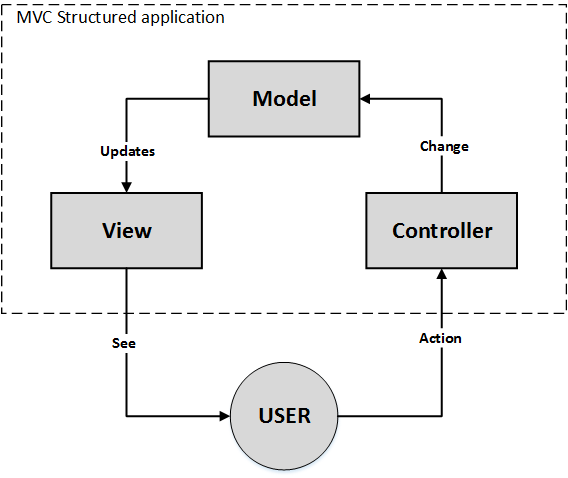
\includegraphics[width=0.7\linewidth]{Data/Control_Software/MVC_general.png}
\caption{Model, View and Controller (MVC) relative to user.}
\label{fig:mvc_general}
\end{figure}

Shown in the Figure \ref{fig:mvc_general} interaction is a classical MVC architecture. There are various realization of this diagram in terms of interaction between three main object types of MVC. The main reasons of it are various application types and their realizations. For instance, in our application this diagram will look like in the Figure \ref{fig:mvc_custom}.

\begin{figure}[ht]\centering
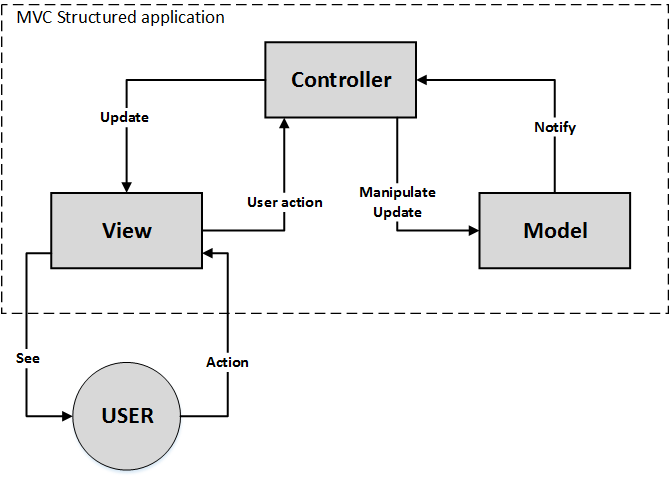
\includegraphics[width=0.7\linewidth]{Data/Control_Software/MVC_custom.png}
\caption{Model, View and Controller (MVC) relative to user.}
\label{fig:mvc_custom}
\end{figure}

Comparing to classical MVC structure from Figure \ref{fig:mvc_general}, the Model do not directly inform/update the View. This information passes through Controller. A controller object acts as the intermediary between the Model and the View. Controllers are often in charge of making sure the views have access to the model objects they need to display and act as the conduit through which views learn about changes to the model. Controller objects can also perform set-up and coordinating tasks for an application and manage the life cycles of other objects \cite{apple_MVC}.

Depending on the application logic and demands, Model, View and Controller follow special properties and rules.

\emph{Model} is central component of the system. It directly manages the data, defines the logic and rules of the application which manipulates the date. Moreover, like in our case, it regulates the interaction between the application and hardware. For instance, there is a Model class \emph{ConradModel} in our application. It is responsible for communication with a relay card for turning on and off vacuum lines. This class completely meet MVC rules as a Model object because it does not depend on any other class, while others depend on it using its possibilities for their functions.

\emph{View} unite all objects responsible for visual part of the application: windows, tabs, labels, forms, buttons, etc. They know how to display the data from the application's model and also give a user the possibility to edit the data. For instance, one task of \emph{AssemblyModuleAssembler} class is to display the information about Vacuum lines of the system, as well as control elements for it. However, it only display the control elements, but not process the user's actions.

\emph{Controller} is mainly responsible for accepting input and processing it, generating commands for the Model or the View. For instance, \emph{ConradManager} provides all necessary functions to control the vacuum lines and to get the current status of it. It is worth noting that very often there is no direct connection between the Model and the View, like it is shown in the classical MVC architecture in the Figure \ref{fig:mvc_general}. Instead of it, the Controller acts as the intermediary between the application's model objects and its view objects.

\subsection{OpenCV library}

A lot of algorithms needed for the application were found in the open-source library~---~OpenCV (\textit{Open Source Computer Vision}). It is a cross-platform library of programming functions mainly oriented on real-time computer vision. It was originally developed by Intel's research center in Nizhny Novgorod (Russia). Later it was supported by Willow Garage and is now maintained by Itseez. The library is free for use under the open-source BSD license~\cite{OpenCV_general}.

OpenCV was designed for computational efficiency and, as was already mentioned, with a strong focus on real-time applications. It is written in optimized C++ and can take advantage of multicore processors. There is also a possibility for further automatic optimization on Intel architecture with Intel's \textit{Integrated Performance Primitives (IPP)} libraries, which consist of low-level optimized routines in many different algorithmic areas~\cite{kaehler2016learning}.

One of the main goals of OpenCV is to provide a simple-to-use computer vision infrastructure that helps people build fairly sophisticated vision applications quickly. In its libraries one can find over 500 functions that span many areas in vision. In the list below one can see main features of the OpenCV library~\cite{Illinois_openCV}:
\begin{itemize}
\setlength\itemsep{-0.5em}
\item Image data manipulation (allocation, release, copying, setting, conversion).
\item Image and video I/O (file and camera based input, image/video file output).
\item Matrix and vector manipulation and linear algebra routines (products, solvers, eigenvalues, SVD).
\item Various dynamic data structures (lists, queues, sets, trees, graphs).
\item Basic image processing (filtering, edge detection, corner detection, sampling and interpolation, color conversion, morphological operations, histograms, image pyramids).
\item Structural analysis (connected components, contour processing, distance transform, various moments, template matching, Hough transform, polygonal approximation, line fitting, ellipse fitting, Delaunay triangulation).
\item Camera calibration (finding and tracking calibration patterns, calibration, fundamental matrix estimation, homography estimation, stereo correspondence).
\item Motion analysis (optical flow, motion segmentation, tracking).
\item Object recognition (eigen-methods, HMM).
\item Basic GUI (display image/video, keyboard and mouse handling, scroll-bars).
\item Image labeling (line, conic, polygon, text drawing).
\end{itemize}

The application of the OpenCV libraries will be described more detailed in the next section.

\section{Pattern recognition}

Pattern recognition is a crucial part of the whole automated assembly system, in particular -- vision subsystem. It provides the software with the information where all the components of the modules are situated in the space and theirs orientation. Within this information the software is able to calculate where to move each component of an assembling module \cite{AutomatedAssembly_tutorial}.

An important task performed by PSAuto is the determination the \emph{location} and \emph{planar orientation}. By definition, planar orientation is the rotational orientation of the sensor in the horizontal (X-Y) plane of the sensors during the assembly process. This is generally achieved in two basic steps: the independent determination of \emph{localised} positions and orientations of the four markers at the corners of the sensor and a global fit to these positions from which the final position and orientation of the entire sensor is extracted \cite{AutomatedAssembly_tutorial}. 

\begin{figure}[ht]\centering
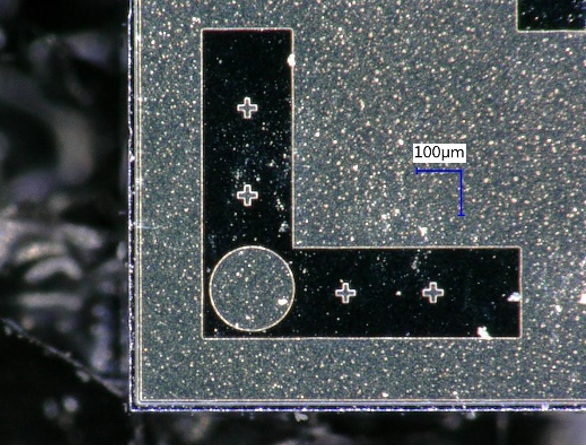
\includegraphics[width=0.7\linewidth]{Data/Control_Software/Fiducial_marker.png}
\caption{Fiducial marker on one of the corner of a PS sensor.}
\label{fig:fiducial_marker}
\end{figure}

This is done by processing the images of \emph{fiducial markers} at the corners of the sensors (Figure \ref{fig:fiducial_marker}) acquired by the vision system with a Pattern Recognition algorithm. The markers are precisely positioned with respect to the strips or pixels or the sensors. Hence precise alignment of the markers ensures precise alignment of the pixels or strips.The algorithm takes raw images as input and returns the position and orientation of fiducial markers located at the corners of the PS sensors. The pattern recognition algorithm utilises the \emph{OpenCV} package. The steps comprising the pattern recognition are now outined:

\begin{enumerate}
\setlength\itemsep{-0.5em}
\item Pre-processing of raw image.
\item Determination of positions and planar orientations of fiducial markers.
\item Location of other corners and extraction of final position and orientation.
\end{enumerate}

\subsection{Pre-processing of raw image}
The raw images from the camera are first converted from colour to black and white which is known as \emph{grayscaling} in OpenCV. The pixels comprising the grayscaled image contain intensity information only in the form of a single number ranging from 0 to 255 describing the darkness of a shade of gray as opposed to the intensity and colour information contained in the pixels of a colour image. As the corner markers are based on simple shapes and not colours, the colour information is not helpful and is thus disregarded. The grayscaled image is then converted to a \emph{binary} image in which each pixel is either black or white in a process known as \emph{thresholding}. Thresholding simply converts each pixel of the image into a white(black) pixel if the intensity of the pixel is above(below) a pre-defined threshold (). Thresholding serves to reduce the differences between images of identical sensors due to random \emph{noise} arising from dust and random differences in the surfaces of the patterned sensors. Examples of grayscaled and thresholded images of the same corner marker of a dummy PS sensor is shown in Figure \ref{fig:threshold}. The optimal threshold will depend on the ambient lighting conditions around the assembly area and and the contrast of the fiducial markings on the sensors. Currently, typical values of threshold are around 90.

\begin{figure}[ht]\centering
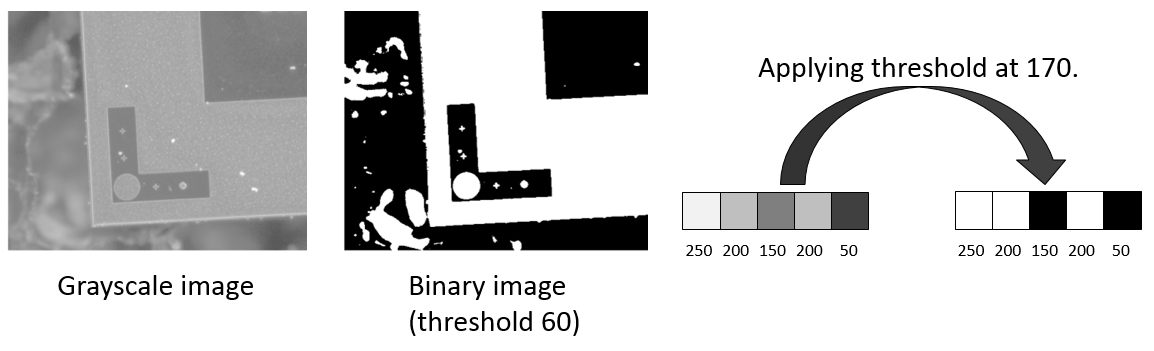
\includegraphics[width=0.9\linewidth]{Data/Control_Software/Threshold.png}
\caption{Threshold application on fiducial marker of dummy PS module.}
\label{fig:threshold}
\end{figure}

\subsection{Determination of positions and planar orientations of fiducial markers.}
The position and orientation of the fiducial marker within the thresholded image is determined using a standard image processing technique known as \emph{template matching}. In template matching, parts of an master image that closely resemble a template image are located. In this case, the master image corresponds to the thresholded image of the fiducial marker and the template image corresponds to a thresholded image of a fiducial marker.

Template matching proceeds by iteratively superimposing the template image at each point of the master image and calculating a metric which describes the similarity of the template image and the portion of the master image with which it coincides. The OpenCV package provides multiple options for the metric. Similar results are observed for each possible metric with the chosen metric based on the normalised squared difference between the intensities of coincident pixels of the master image and superimposed template:


\begin{center}
$R(x,y)=\dfrac{\sum_{x',y'}^{}(T(x',y')-I(x+x',y+y'))^{2}}{\sum_{x',y'}^{}\sqrt{\sum_{x',y'}^{}T(x',y')^{2}\cdot\sum_{x',y'}^{}I(x+x',y+y')^{2}}}$
\end{center}
where I denotes \emph{master image}, T -- \emph{template image} and R -- \emph{resultant metric}.

This metric is referred to as CV\_TM\_SQDIFF\_NORMED in OpenCV. The point in the master image where the metric reaches a minimum represents the most probable location of the fiducial marker. In Figure \ref{fig:template_matching} the determination of marker position with template matching and its result using images of the dummy sensor is illustrated. The most probable location of the marker as determined by the algorithm is indicated by the white rectangle. The observed location matches closely with expectation.

\begin{figure}[ht]\centering
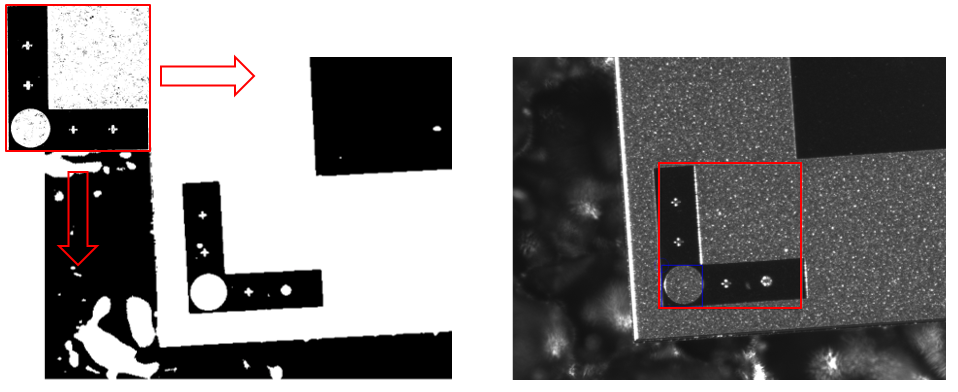
\includegraphics[width=0.9\linewidth]{Data/Control_Software/Template_matching.png}
\caption{The technique of template matching is illustrated on the left image. The red arrows indicate the iterative calculation of a metric at each point of the master image. The result of a template matching routine on using test images is shown on the right image. The most probable location of the marker in the master image is outlined by the red rectangle.}
\label{fig:template_matching}
\end{figure}

In order to deduce the orientation of the marker in the plane transverse to the optical axis of the camera, the matching procedure is repeated iteratively with different rotational transformations applied to the master image. For each iteration, the minimal value of the metric is recorded with the minimal metric value across all iterations denoted as $\alpha$. The planar orientation of the sensor is estimated as $-\alpha$. In Figure \ref{fig:template_rotation} a schematic illustrating the determination of the orientation is shown. A graph of the resultant minimised metric values versus the size of the angular transformation applied to the master image is shown on the right image of the Figure \ref{fig:template_rotation}. The graph corresponds to a test extraction performed with images of a dummy sensor where the sensor in the master image had a planar orientation of $\approx$ 3.5 degrees. A clear minimum is observed at $\approx$ 3.5 demonstrating the method's validity. More precise determination of the sensor orientation can be achieved when factors such as ambient light conditions, image focus and marker design are further optimised. The best accuracy reached during tests was $\approx$ 0.025 degrees.

\begin{figure}[ht]\centering
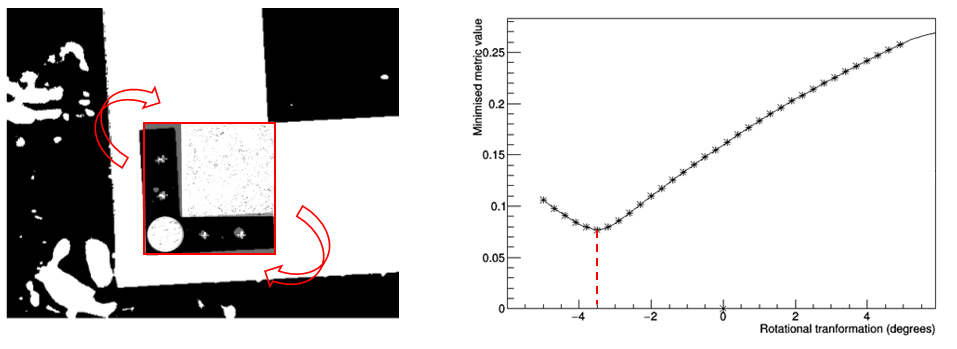
\includegraphics[width=0.9\linewidth]{Data/Control_Software/Template_rotation.png}
\caption{A schematic illustrating the estimation of the sensors planar orientation is shown on the left image. The red arrows indicate the iterative rotational transformations applied to the master image. graph of the minimised metric value versus the angular transformation applied to the master image is shown on the right image. A clear minimum at $\approx$ 3.5 degrees is observed.}
\label{fig:template_rotation}
\end{figure}

\subsection{Location of other corners and extraction of final position and orientation.}
The procedure described in step 2 is repeated at each sensor corner. The planar orientations determined at given corner are used to set the direction of movement needed for the motion stage to automatically travel to an adjacent corner. The final position and orientation of the sensor is determined by a $\chi^{2}$ fit to the four (x,z) points. The orientation determined from the fit is cross-checked with the estimations of the orientation at the corners which accuracy could be not far from $\chi^{2}$ deduced. If there is agreement between the fit and four corner orientations, the fit results are used.

\section{Application functionality}

\subsection{Autofocus}

\subsection{Acquire image}

\subsection{Threshold tuner}

\subsection{Motion manager}



%\subsection{A Subsection}
